% Template para Proposta e TCC da EST/UEA -
% Padrão para os cursos do Núcleo de Computação
%
% Elaborado por Elloá B. Guedes
% Adaptado da versão elaborada por:
%                   Jucimar Maia Jr.
%
% Versão 1.3 - 15 de julho de 2022
%
\documentclass[a4paper,titlepage,12pt]{report}


\usepackage[utf8]{inputenc}
\usepackage[OT1]{fontenc}
\usepackage{ae}
\usepackage[brazil]{babel}
\usepackage{a4wide}
\usepackage{comment}
\usepackage[pdftex]{graphicx,color}
\usepackage{graphics}
\usepackage{cite}
\usepackage{longtable}
\usepackage{float}
\usepackage{fancyvrb}
\usepackage{fancyhdr}
\usepackage{setspace}
\usepackage{amsmath}
\usepackage{lscape}
\usepackage{textcase}
\usepackage{anysize}
\usepackage{setspace}
\usepackage{booktabs}
\usepackage{url}
\usepackage{subfig}
\usepackage{cite}
\usepackage[alf]{abntex2cite}
\usepackage{pdfpages}

\marginsize{20mm}{20mm}{20mm}{15mm}


%% Cabeçalhos
\renewcommand{\topfraction}{1}
\renewcommand{\bottomfraction}{1}
\renewcommand{\floatpagefraction}{1}
\renewcommand{\textfraction}{0}
%\renewcommand{\baselinestretch}{2}
\doublespacing %espaçamento duplo
\sloppy

%% Nomes
\floatstyle{plain}  %%% tipos: plain, boxed, ruled
\newfloat{codigo}{tbp}{lop}[section]
\floatname{codigo}{Código}

%%% nome para ser usado no sumário

\newcommand{\listofcodename}{Lista de C\'{o}digos}



% RESUMO ----------------------------------------------------------------------------------------------------------------------------------------------------------------------

\newcommand{\resumo}[1]{
\begin{center} \LARGE \bf Resumo \end{center}

\vskip 4em
\input{#1}

\newpage

}

% ABSTRACT ----------------------------------------------------------------------------------------------------------------------------------------------------------------------

\newcommand{\abstractt}[1]{
\begin{center} \LARGE \bf Abstract \end{center}

\vskip 4em
\input{#1}

\newpage

}

% AGRADECIMENTOS ----------------------------------------------------------------------------------------------------------------------------------------------------------------------
\newcommand{\agradecimentos}[1]{
\chapter*{Agradecimentos} % Título alinhado à esquerda
\input{#1}
\newpage
}

% EPÍGRAFE ----------------------------------------------------------------------------------------------------------------------------------------------------------------------
\newcommand{\epigrafe}[1]{
\chapter*{Epígrafe} % Título alinhado à esquerda
\vspace*{\fill} % Preenche o espaço vertical até o final da página
\begin{flushright} % Alinha o texto à direita
\textit{#1} \\[1em] % Texto em itálico com espaçamento
\end{flushright}
\vspace*{-0.5cm} % Ajusta o posicionamento para ficar mais próximo ao canto inferior direito
\newpage
}

% Sumário -----------
\newcommand{\sumario}{
\renewcommand{\contentsname}{Sum\'{a}rio}
\tableofcontents
\addcontentsline{toc}{chapter}{\listtablename}
\listoftables

\newpage
\addcontentsline{toc}{chapter}{\listfigurename}
\listoffigures
%\addcontentsline{toc}{chapter}{\listofcodename}
% \listof{codigo}{\listofcodename}  % Lista de Códigos

\clearpage
}

\pagestyle{plain}

\newcommand{\folhaRosto}[5]{

\thispagestyle{empty}
\begin{center}
\textbf{\\[0.4em]\MakeUppercase{#2} \\[5cm]}
\textbf{\MakeUppercase{#1}\\[96pt]}

\end{center}

\hspace*{8cm}
\begin{minipage}{8cm}
Trabalho de Conclus\~{a}o de Curso
apresentado \`{a} banca avaliadora do Curso de Engenharia de Computa\c{c}\~{a}o, da
Escola Superior de Tecnologia, da Universidade do Estado do Amazonas, como
pr\'e-requisito para obten\c{c}\~{a}o do t\'{\i}tulo de Engenheiro de Computa\c{c}\~{a}o.\\[40pt]
\end{minipage}

\begin{center}
Orientador(a): #3 \\[12ex]
Manaus -- #4 -- #5\\
\end{center}


\pagenumbering{roman}
\newpage
}




%% Preencha aqui os seguintes dados
\def \titulo{BURI : Sistema Android Embarcado de monitoramento da qualidade do ar em ambiente residencial}
\def \orientador{Prof. Msc. Jonathas Silva dos Santos}
\def \nome{Adevan Neves Santos}
\def \mes{Agosto}
\def \ano{2024}

\begin{document}

\folhaRosto{\titulo}{\nome}{\orientador}{\mes}{\ano}

% Edite os seguintes arquivos para alterar as informações necessárias
\begin{center} \LARGE \bf Ficha Catalográfica \end{center}


\begin{enumerate}
    \item Estas instruções \textbf{não} devem ser entregues aos avaliadores do trabalho nas ocasiões dos TCCs 1 e 2. Portanto, comente a linha que importa este arquivo;
    \item A ficha catalográfica deve ser elaborada após a defesa do TCC2, quando você concluir as correções sugeridas pela banca e validar a versão final com o/a professor(a) orientador(a);
    \item Acessar \url{http://repositorioinstitucional.uea.edu.br:8080/ficha/ficha_catalografica.php} e preencher as informações requeridas para elaborar a ficha catalográfica;
    \item Incluir o pdf gerado na subpasta \emph{source} com o nome \texttt{ficha.pdf};
    \item Apagar todo o conteúdo deste arquivo e deixar apenas o comando a seguir:
    \begin{verbatim}
        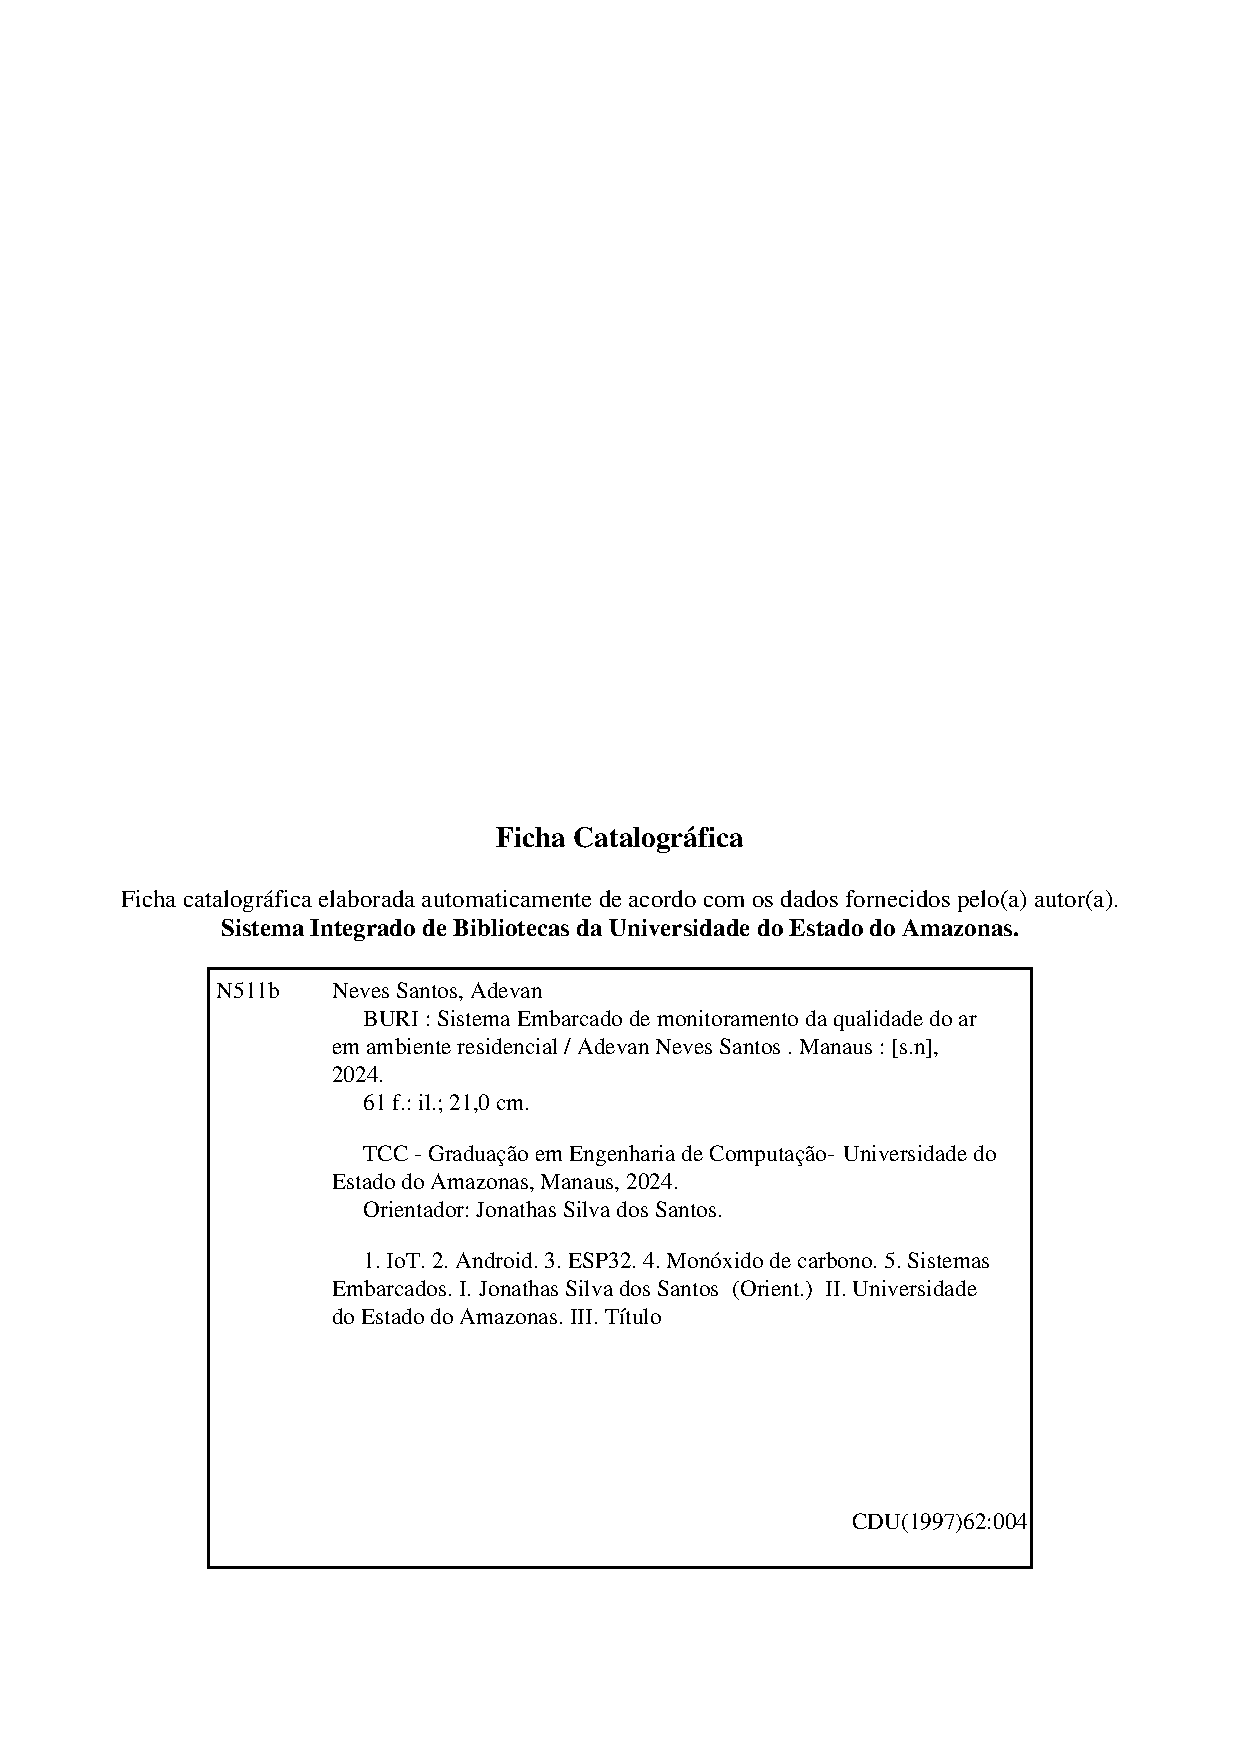
\includepdf[pages=-]{./source/ficha.pdf}
    \end{verbatim}
\end{enumerate}

\newpage

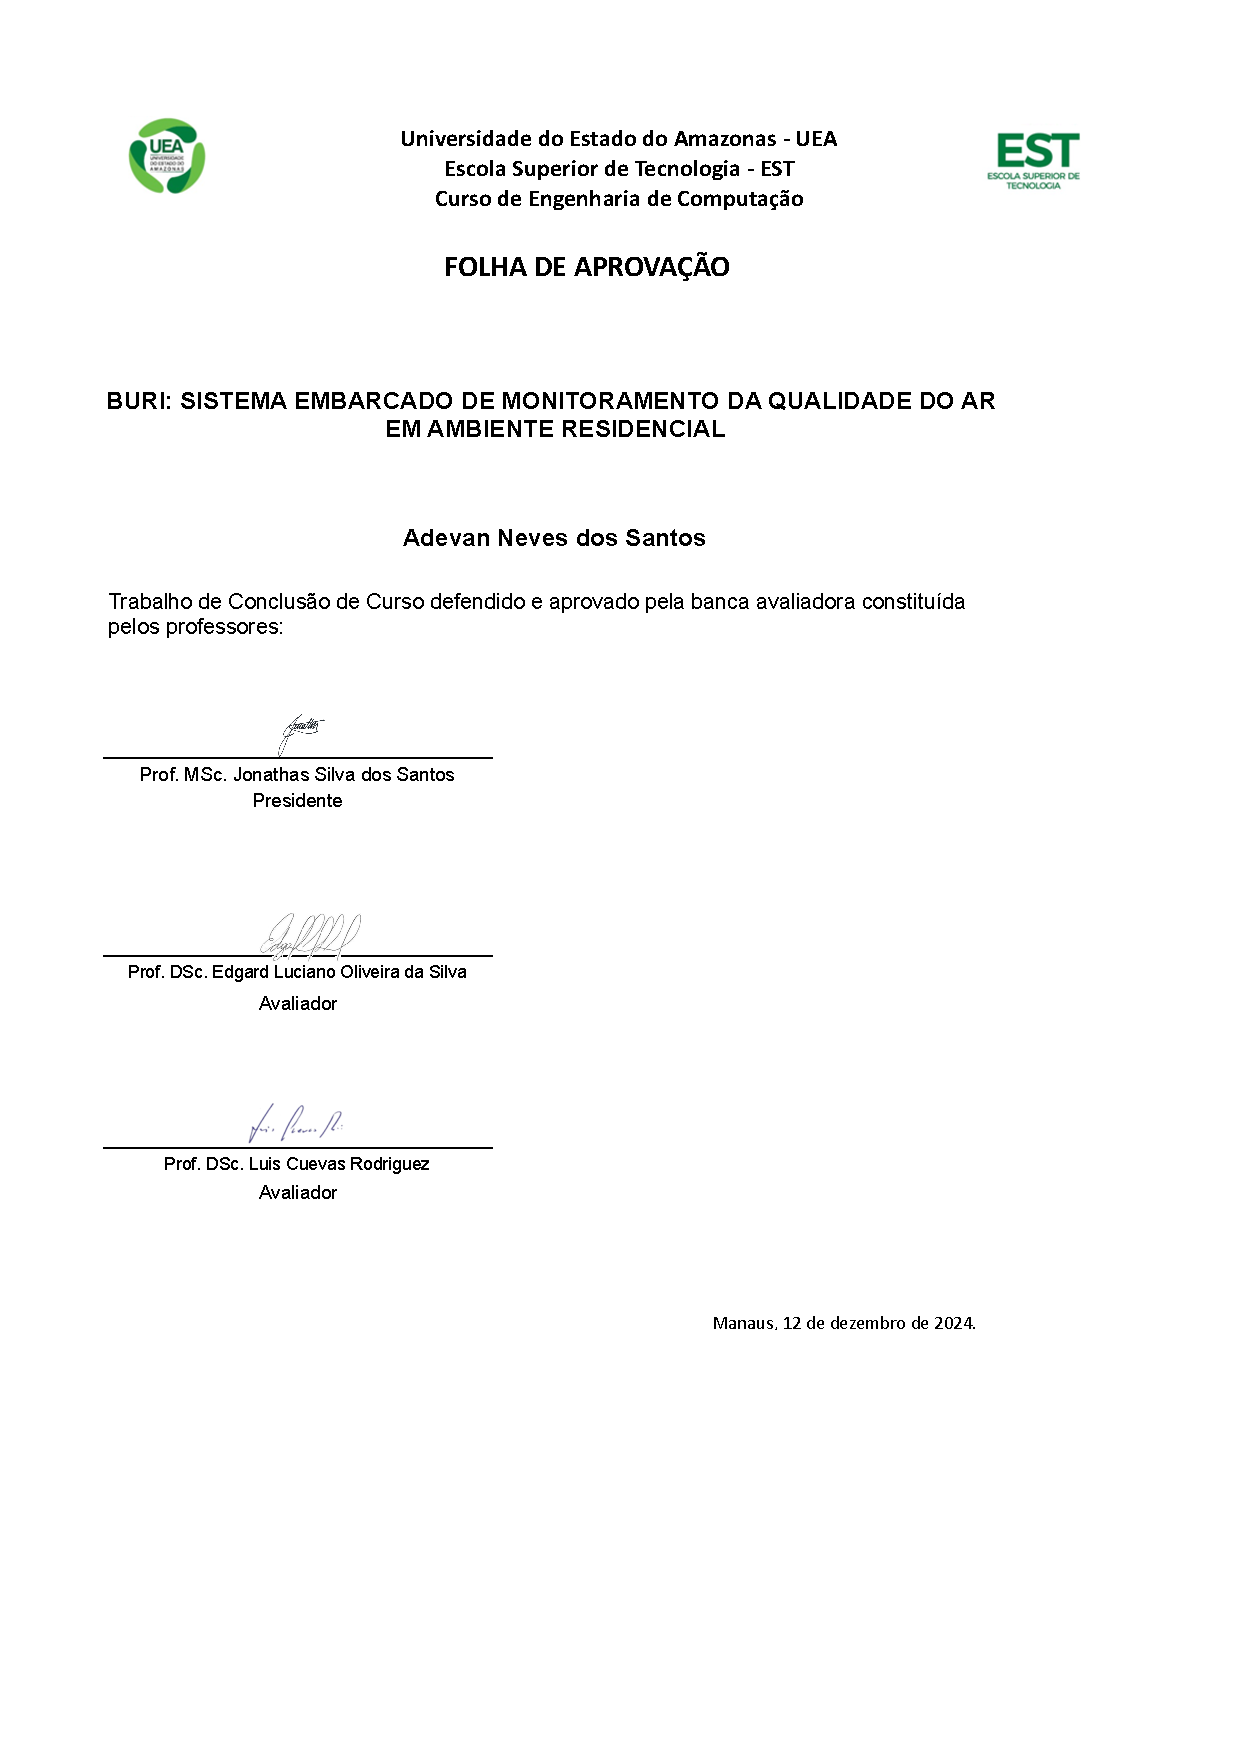
\includepdf[pages=-]{./source/assinaturas.pdf}


% Indique onde esta o arquivo do resumo
\resumo{./files/resumo.tex}
% Idem para o abstract
\abstractt{./files/abstract.tex}


\sumario

% Configuração de cabeçalhos
\pagestyle{fancy}
\renewcommand{\chaptermark}[1]{\markboth{#1}{}}
\renewcommand{\sectionmark}[1]{\markright{#1}}
\renewcommand{\headrulewidth}{0.5pt}
\newcommand{\rom}{\fontfamily{cmr}\fontseries{m}\fontsize{10}{12}\selectfont}
\fancyhf{} \fancyhead[LE,RO]{\rom\thepage}
\fancyhead[LO]{\rom\rightmark} \fancyhead[RE]{\rom\leftmark}
\fancypagestyle{plain}{
    \fancyhead{} % get rid of headers
    \renewcommand{\headrulewidth}{0pt} % and the line
 }


\pagenumbering{arabic}



% Seus capítulos vão aqui --------
\chapter{Introdução}

Em outubro de 2023, Manaus liderou a lista das cidades com a pior qualidade do ar no mundo, apresentando nuvens 
de fumaça em alguns dias do mês. Segundo a prefeitura da capital amazonense, essa situação foi resultado da 
intensa onda de queimadas na região \cite{G1-ar-manaus}. Diante do cenário descrito, uma preocupação relevante 
é a intoxicação por inalação de gases asfixiantes, como o monóxido de carbono (CO). O gás, presente no ar devido à combustão 
incompleta de materiais ricos em carbono, é uma substância tóxica, incolor e inodora, que atua no organismo da 
seguinte forma: ao se ligar quimicamente à hemoglobina, proteína no sangue responsável pelo transporte de oxigênio, com uma afinidade de 
200 a 300 vezes maior que a ligação do oxigênio ($O_{2}$), o monóxido de carbono reduz a eficiência do transporte de oxigênio no organismo e 
pode levar a óbito caso haja exposição prolongada e em altas quantidades \cite{carbon-monoxide-poisoning-varon}.

No ambiente doméstico, as fontes mais comuns do gás CO são: aquecedores, fogões, automóveis 
em garagens pouco ventiladas, entre outros. Outro fator de risco é o vazamento devido ao mau 
uso e/ou à falta de manutenção dos equipamentos, pois a detecção do gás antes do início dos 
sintomas é prejudicada na ausência de equipamentos de medição \cite{bio-sufocantes-hernandez2022}. Portanto, 
decidiu-se abordar a problemática por meio de um sistema embarcado, com foco na emissão de 
alerta de risco aos ocupantes. O projeto de trabalho de conclusão de curso consiste na elaboração e 
desenvolvimento de um protótipo de \textit{hardware}, em conjunto com o \textit{software} necessário na 
interação do usuário com os outros módulos do sistema. 

\section{Objetivos}

O objetivo geral do trabalho é oferecer uma solução de sistema embarcado para o monitoramento da qualidade do ar em ambiente residencial, com 
ênfase na coleta de dados e identificação de condições de risco, pois proporcionar aos moradores informações cruciais sobre a qualidade do ar interno 
contribui na adoção de medidas preventivas.

Portanto, para alcançar o objetivo geral, é necessário cumprir os seguintes objetivos específicos:
\begin{itemize}
    \item Elaborar pesquisa com usuários e avaliação do sistema;
    \item Coletar, compreender e tratar as informações dos sensores de: monóxido de carbono, temperatura e umidade do ar;
    \item Construir o protótipo do dispositivo embarcado;
    \item Realizar a comunicação entre o dispositivo e os demais módulos da aplicação;
    \item Desenvolver a API de dados e eventos, assim como a interface do sistema com o usuário;
\end{itemize}

\section{Justificativa}

O projeto visa contribuir para o monitoramento e detecção de riscos de intoxicação de gás em residências, cujo 
impacto se manifesta na prevenção de acidentes, tomada de decisão com apoio de dados e também na automatização 
de sinais de alerta. Outro ponto de destaque da importância desse trabalho diz respeito ao risco de morte por asfixia 
que a substância monóxido de carbono possui, pois sua presença não é detectada pelo olfato humano e o tempo de exposição é um 
fator determinante para os efeitos na saúde. 

A diminuição no fornecimento de oxigênio causa consequências graves ao organismo, indo desde sintomas brandos como náusea e dores de 
cabeça até casos mais sérios como, por exemplo, lesão neurológica e disritmia cardíaca \cite{carbon-monoxide-poisoning-varon}. Esta perspectiva enriquece a 
contribuição do trabalho no campo de IoT e ressalta a importância do uso de sistemas inteligentes para o monitoramento ambiental.  

\section{Metodologia}

A metologia de trabalho baseia-se no \textit{embedded design life cycle diagram} \cite{system-design-IOT}. O fluxo de atividades possui vantagem no 
particionamento de atividades em \textit{hardware} (HW) e \textit{software} (SW), ao favorecer 
a execução de  múltiplas tarefas no mesmo projeto em concordância com a entrega parcial, sendo positivo para sistemas embarcados e 
suas características intrínsecas, como alto acoplamento, dependência entre componentes eletrônicos e a leitura de dados pelo software, além da própria limitação de 
poder computacional oferecido pelos dispositivos. A execução simultânea de atividades em 
duas áreas permite a validação de funcionalidades do sistema nas entregas incrementais e otimização do 
processo de desenvolvimento, porém sua complexidade exige um maior cuidado com a execução em ordem de tarefas. Portanto, o método original possui 7 fases principais:  

\begin{enumerate}
    \item Especificação do produto;
    \item Particionamento em componentes de \textit{hardware} e \textit{software};
    \item Iteração e refinamento das funcionalidades;
    \item Atividades de \textit{hardware} e \textit{software};
    \item Integração de componentes;
    \item Testes de aceitação e lançamento do produto;
    \item Manutenção e atualização do produto final;
\end{enumerate}

Contudo, o método original trata do desenvolvimento de um produto (e não de uma pesquisa acadêmica). Dito isso, o processo sofreu as seguintes 
adaptações ao contexto da universidade: a primeira fase deverá conter a pesquisa de trabalhos relacionados, domínio do problema e questionários com potenciais usuários, enquanto sua última etapa trata de documentação e escrita 
da monografia, como resultado do trabalho de conclusão de curso. Portanto, a seguinte figura demonstra a metodologia utilizada na execução do sistema BURI: 

\begin{figure}[ht]
\centering
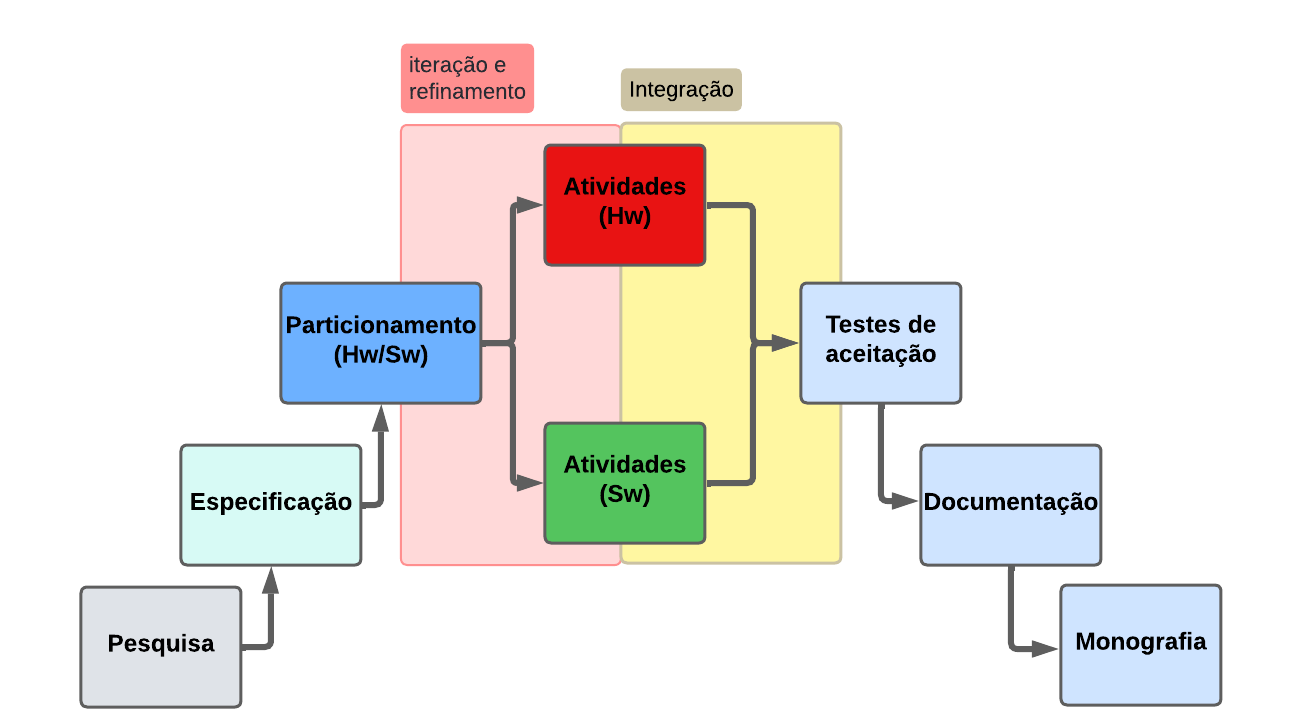
\includegraphics[width=.75\textwidth]{img/diagrama-metodologia.png}
\caption{Fluxo de atividades. Fonte: Elaboração própria com base  em \cite{system-design-IOT}}\label{figMetodologia}
\end{figure}


\chapter{Fundamentação Teórica}

Este capítulo detalha os principais conceitos e tecnologias aplicados no projeto: Internet das Coisas, sistemas distribuídos, protocolo HTTP, AOSP, desenvolvimento Android e ESP32 com NodeMCU. Portanto, 
a seguinte seção aborda como os conceitos citados contribuíram para o desenvolvimento deste trabalho de conclusão de curso, possibilitando
ao leitor uma visão geral das competências necessárias em sua execução. 

\section{Internet das Coisas}

O termo \textit{Internet das Coisas} (\textit{IoT}, da expressão em inglês \textit{Internet of Things}) foi utilizado primeiramente em 1999 pelo então pesquisador do \textit{Massachusetts Institute of Technology} (MIT) Kevin Asthon em uma apresentação na Procter \& Gamble (P\&G) sobre a tecnologia do \textit{Radio Frequency Identification} (RFID). O RFID é uma tecnologia utilizada para a identificação e rastreamento de objetos, animais ou pessoas via ondas de rádio. Portanto, Asthon pontuou a possibilidade de utilizar tal ferramenta para gerenciar a cadeia de suprimentos da empresa, pois sua capacidade de ler vários emissores simultaneamente, sem a necessidade de linha de visão direta entre o leitor e a tag (ao contrário da tecnologia de códigos de barras) torna o monitoramento de cada produto nos distintos pontos de transporte mais fino e mensurável. A ideia do autor 
é que os próprios objetos tenham a capacidade de gerar os dados e reagir aos estímulos do ambiente \cite{iot-first-definition}.

\textit{IoT} possui muitas definições. Embora não haja um consenso convergente para uma definição única, podemos discutir sobre seu impacto na sociedade atual e aspectos importantes que toda solução na área possui. No livro \textit{The Internet  of Things}, escrito por Samuel Greengard, o tema é abordado como um evento disruptivo, onde a linha que separa o humano e a tecnologia se torna cada vez menos visível, porém o texto aborda não somente a capacidade de conexão entre as máquinas, e sim a autonomia e "inteligência" cada vez maior dos sistemas embarcados \cite[pp. 17]{book-iot}. Essa visão de tecnologia integrada no cotidiano é o conceito que o autor Mark Weiser aborda no seu artigo denominadao \textit{The Computer for the 21st Century}. A computação ubíqua é o processo de tornar os computadores ``invisíveis'' aos nossos olhos, desenvolvendo a comunicação com tais ferramentas o mais próximo possível da forma humana, ou seja, o dispositivo tem conexão com a rede e responde aos estímulos do usuário por interfaces naturais, por exemplo, a fala e gestos com as mãos \cite{ubiquitous-computing}.

Portanto, o significado mais comum de \textit{IoT} talvez seja a de dispositivos eletrônicos conectados na internet, permitindo enviar e receber dados do ambiente real. No entanto, apenas conectar dispositivos não é uma solução em Internet das Coisas, pois essa área envolve o uso de protocolos de comunicação, eletrônica de baixo consumo energético, plataformas em nuvens e outras inúmeras áreas do conhecimento. Os dados coletados de sensores atuam como combustível para a execução de um fluxo de tomada de decisão \cite{iot-cycle}. 

\begin{figure}[ht]
    \centering
    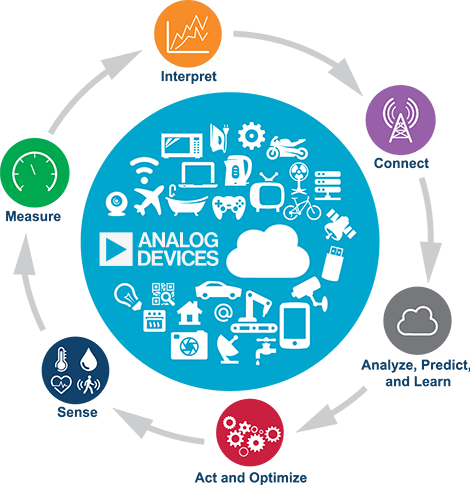
\includegraphics[width=.45\textwidth]{img/iot-cycle.png}
    \caption{Ciclo de IoT. Fonte:\cite{iot-cycle}}\label{figIoTCycle}
\end{figure}

Atualmente, a coleta de dados e uso de ferramentas de análise são o principal recursos de empresas competitivas no gerenciamento de suas atividades. Com o avanço da área de telecomunicações, as organizações têm potencial de transformar grandes volumes de dados em \textit{insights} poderosos, que orientam a tomada de decisões da equipe de gestão. Portanto, a Internet das Coisas representa uma tendência forte e disruptiva na sociedade.

Por exemplo, a Amazon\textsuperscript{\textregistered}, uma das maiores empresas de comércio eletrônico no mundo, anunciou em 2022 o lançamento do robô \textit{Sparrow}, cuja função é manipular objetos em esteiras e realizar o empacotamento
com destreza comparável à de seres humanos. Em suas fábricas, existe um crescente uso de tecnologias de ponta, como robôs autônomos e inteligência artificial, para maximizar as suas entregas em um mercado competitivo \cite{amazon-robos}.

\section{Sistemas Distribuídos}

``Um sistema distribuído é aquele no qual os componentes localizados em computadores interligados em rede se comunicam e coordenam suas ações apenas passando mensagens.'' \cite[pp. 1]{sistemas-distribuidos-coulouris2013}.
A definição apresentada pelo autor leva em conta dois importantes fatores: o primeiro é representado pela comunicação via rede de computadores, e o segundo está relacionado ao provisionamento de um serviço.
O mundo atual oferece inúmeros exemplos da importância dos sistemas distribuídos no desenvolvimento socioeconômico: a modalidade de educação à distância \cite{mec-ead}, no qual serviços web e compartilhamento
multimídia são responsáveis por possibilitar o acesso ao ensino de qualidade ao público distante fisicamente dos grandes centros de ensinos, como, por exemplo, cidades do interior ou comunidades ribeirinhas; o comércio digital, onde a arquitetura do sistema deve suportar picos de acesso em determinados períodos do ano e controle
de concorrência na compra de produtos, deve-se ao crescimento do seguimento de \textit{e-Commerce},
resultou em um faturamento superior à R\$ 180 bilhões de reais em 2023 no Brasil, de acordo com dados da Associação Brasileira de Comércio Eletrônico \cite{abcomm-ecomerce}; e redes \textit{blockchain}, pois as transações distribuídas devem ser auditáveis e transparentes, além do funcionamento descentralizado \cite{juliana-blockchain}, exemplo 
das criptomoedas, pois a tecnologia permite a transferência de recursos e o armazenamento de todas as operações.  

Portanto, o sistema distribuído tem foco no compartilhamento de recursos. Na web, a implementação de arquitetura mais comum é o modelo cliente/servidor, pois
um número grande de aplicações utiliza essa premissa, por exemplo, plataformas de redes sociais, jogos online e serviços bancários.
Ao nível do Sistema Operacional, a comunicação entre processos executados em diferentes computadores interligados em rede é essencial para o gerenciamento e acesso aos recursos distribuídos.
Nesse contexto, um cliente, que pode ser um processo ou aplicativo, realiza uma solicitação ao servidor para acessar ou manipular um recurso, como arquivos, impressoras, ou mesmo capacidade de processamento. O servidor, 
ao receber essa solicitação, desencadeia uma série de operações internas, que podem incluir desde a autenticação do cliente até a busca de dados em um banco de dados distribuído. Em seguida, o servidor 
retorna o resultado ao cliente em espera, completando o ciclo de comunicação do tipo requisição/resposta \cite[pp. 16]{sistemas-distribuidos-coulouris2013}.

\section{Protocolo HTTP}

O HTPP (do inglês \textit{HyperText Transfer Protocol})

\section{AOSP}

AOSP é coisa e tal

\section{Desenvolvimento Android}

Android é coisa e tal 

\section{ESP32 e NodeMCU}
\chapter{Exemplo}

\section{Tabela com o Pacote Booktabs}

Um exemplo de tabela com o pacote booktabs pode ser visto na Tabela \ref{tabela:exemplo}. A explicação das tabelas sempre vem em cima e esse padrão deve ser respeitado. A numeração é automática e a inserção no índice também. Legal né? \cite{Bennett:QuantumInformationSurvey}

Basta quebrar uma linha para criar um novo parágrafo. Neste parágrafo vou contar que tabelas no \LaTeX dão um pouco de trabalho, mas nada que com paciência não se resolva. Veja os links com dicas que coloquei nos comentários do arquivo \texttt{index.tex}.

\begin{table}[ht!]
\caption{Esta é uma tabela básica em \LaTeX com o pacote booktabs.} \label{tabela:exemplo}
\center{
\begin{tabular}{cccc}
\toprule
Parte 1 & Parte 2 & Parte 3 & Parte 4\\
\midrule
0,415 & 1,365 & 1,98 & 2,05\\
1,36  & 45,5  & 7,98 & 3,01\\
2,36  & 1,35  & 0,15 & 5,32\\
\bottomrule
\end{tabular}}
\end{table}



\section{Inserção de Figuras}

Você pode inserir figuras JPG no \LaTeX! Veja o caso da Figura \ref{fig:exemplo}. Se você quiser outras configurações e dicas, veja o seguinte endereço: \url{http://en.wikibooks.org/wiki/LaTeX/Floats,_Figures_and_Captions}.

A explicação da figura sempre vem embaixo da mesma. Isto aqui é um novo parágrafo apenas para ilustrar a idéia geral de como escrever.

\begin{figure}[H]
\centering
\caption{Um exemplo de figura JPG inserida no \LaTeX.} \label{fig:exemplo}
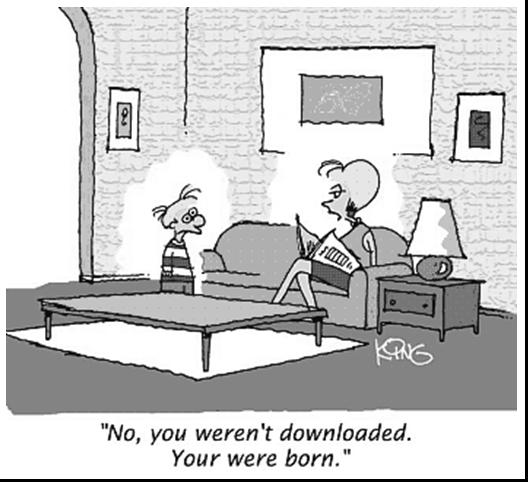
\includegraphics[width=0.4\textwidth]{./img/exemplo.jpg}\\
\small{Elaborado pelo autor.}
\end{figure}

Pode inserir várias figuras lado a lado também. Um exemplo está reproduzido a seguir.

\begin{figure}[H]
  \centering
  \caption{Canal clássico cuja obtenção da capacidade erro-zero é não-trivial.}
  \subfloat[\ ]{\label{fig:exG5}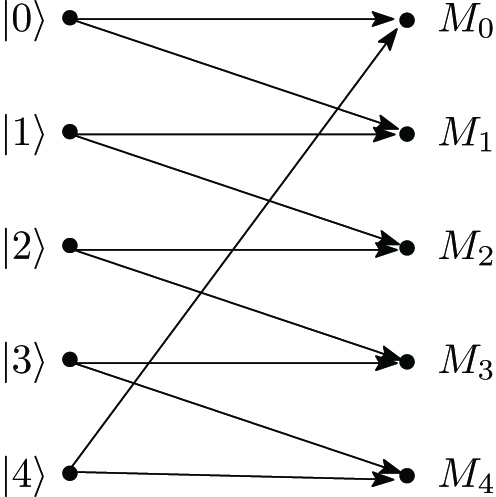
\includegraphics[width=0.3\textwidth]{./img/001}}
  \hspace{0.5cm}
  \subfloat[\ ]{\label{fig:exG52}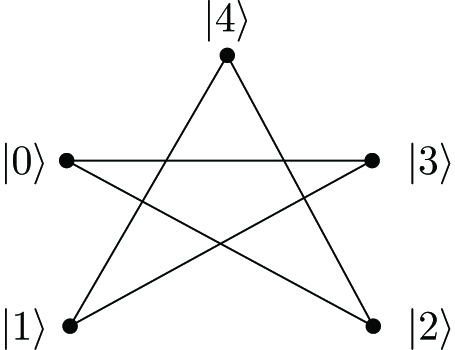
\includegraphics[width=0.3\textwidth]{./img/002}}
  \hspace{0.5cm}
  \subfloat[\ ]{\label{fig:exG53}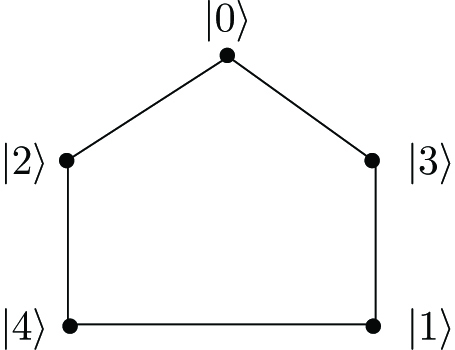
\includegraphics[width=0.3\textwidth]{./img/003}}\\
  \small{Elaborado por Bacon}
\end{figure}

\section{Referências Bibliográficas no Padrão ABNT}

Para gerar versões corretas do \textsc{Bib}\TeX das suas referências, recomenda-se usar o DOI no caso de artigos e o ISBN no caso de livros. Em posse dessas informações, consulte os seguintes links:

\begin{enumerate}
    \item \url{https://www.bibtex.com/c/doi-to-bibtex-converter/}
    \item \url{https://www.bibtex.com/c/isbn-to-bibtex-converter/}
    \item \url{http://doi-to-bibtex-converter.herokuapp.com/}
    \item \url{https://www.doi2bib.org/}
\end{enumerate}

Para saber mais sobre os tipos de referências \textsc{Bib}\TeX e seus significados, consultar a documentação oficial em \url{https://www.bibtex.com/e/entry-types/}.

Este template está integrado com o pacote \texttt{abnt2cite} que produz as referências no padrão ABNT NBR 6023.

\chapter{Resultados e Discussão}



\section{Análise dos questionários}\label{questionario}

\section{Teste do sistema de alerta}\label{alerta}

\section{Comparação técnica com trabalhos similares}\label{comparacao}



% Referência segundo o padrão ABNT
% Edite este arquivo e inclua suas referências segundo a notação do Bibtex
\bibliography{ref}



\end{document}
